\documentclass[11pt, a4paper]{arbeitsblatt}

\ladeModule{theme,qrcodes}
\aboptionen{
	name 		= {J. Neugebauer},
	kuerzel 	= {Ngb},
	titel 		= {Zusammenfassung Sortieralgorithmen},
	reihe 		= {Suchen und Sortieren},
	fach 		= {Informatik},
	kurs 		= {EF},
	nummer 		= {IV.4},
	lizenz 		= {cc-by-nc-sa-4},
	version 	= {2021-05-31},
}

\begin{document}
\ReiheTitel

\begin{wrapfix}
\begin{wrapfigure}[12]{r}{0pt}
	\qrcode{https://scratch.mit.edu/projects/536837143}
\end{wrapfigure}
\textcolor{secondary}{\bfseries 1.} Implementierung des Bubblesort-Algorithmus in Scratch:

\begin{center}
	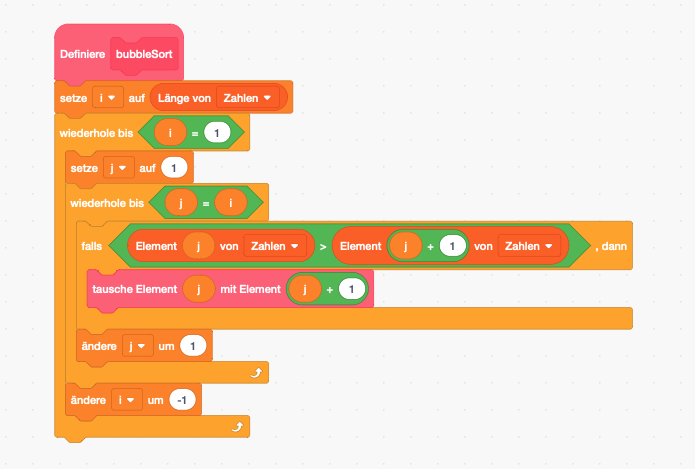
\includegraphics[width=.8\linewidth]{EF-AB.IV.4-Loesung_Bubblesort.png}
\end{center}
\end{wrapfix}

\begin{wrapfix}
\begin{wrapfigure}[12]{r}{0pt}
	\qrcode{https://scratch.mit.edu/projects/536840268}
\end{wrapfigure}
\textcolor{secondary}{\bfseries 2.} Untersuchung der \emph{Laufzeit} für verschiedene Arraylängen:

\begin{multicols}{2}\small
	\begin{tabular}{cc}
		\textbf{Anzahl Elemente} & \textbf{Zeit (s)} \\
		10 & 0,033 \\
		178 & 0,071 \\extern
		370 & 0,171 \\
		649 & 0,473 \\
		1033 & 1,146 \\
		1329 & 1,876 \\
		1756 & 3,11 \\
		2288 & 5,158 \\
		3143 & 9,795 \\
		4176 & 16,941 \\
		5000 & 25,233 \\
	\end{tabular}

	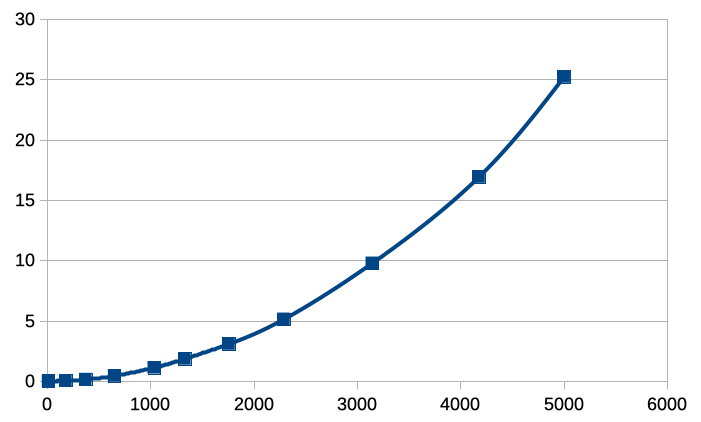
\includegraphics[width=\linewidth]{EF-AB.IV.4-Bubblesort_Chart.png}
\end{multicols}
\end{wrapfix}

\textcolor{secondary}{\bfseries 3.} Ergebnis:

Der Bubblesort ist ein \textbf{quadratisches} Sortierverfahren, das bedeutet seine Laufzeit nimmt
quadratisch mit der Länge des Arrays zu (doppelte Datenmenge $\longrightarrow$ vierfache Laufzeit).
Die Messpunkte können mit einer quadratischen Funktion ungefähr angenährt werden.

\end{document}
